\section{Deployment and User Study}
\label{sec:user-study}

% We implemented a small-scale version of the system and ran a user study in order to demonstrate the system's feasibility.
% The number of participants was too small for any broad conclusions, but we present results for completeness.

We now describe in detail how such a system could be implemented.
We additionally discuss a small-scale deployment and user study we ran in order to demonstrate the system's feasibility.

\subsection{Implementation}
\label{subsec:implementation}
An implementation consists of the five components described in section~\ref{subsec:design}:
a keyword server, a location blacklist module, a network blocking module, an information market, and an access module.
% An implementation consists of several components: Software on the device, in order to hold a user's blacklist and report locations; a web server, to report keywords given a certain lat-long and store users' non-blacklisted locations; and a blocking module, to prevent information leakage.
% Our user study additionally included a web interface to publicly display all users' non-blacklisted locations.
% An Android application, which held a user's blacklist and reported locations; a web server, which reported keywords given a certain lat-long and stored users' non-blacklisted locations; and a web interface, which publicly displayed all users' non-blacklisted locations.

% (i) a keyword server which maps keywords to physical locations
Our \textbf{keyword server} used Yelp's API.
Each time a device uploaded a lat-long to the server, we queried Yelp to find the categories of each location within 50 meters.
This is a possible area for improvement; in future work, the radius of a query could change depending on an estimate of the device's current accuracy or a user's privacy preferences.
The categories were then sent to the device.

Future implementations could likewise map locations to keywords by reusing online services such as Yelp, Google Places, and Foursquare.
% This mapping can be obtained by gathering information from existing sites like Yelp, Google Places, or Foursquare.
A ``folksonomy" approach can be used where users label a map over time, possibly receiving incentive. To encourage tagging of privacy-sensitive locations, the system can allow anonymous tagging. 
% Instead of 
% It may denote a point of interest where users ``check in" (as in services like Foursquare) or alternatively it may represent a certain geographical area (defined using lat-longs or the coverage of a given cell tower).
% Usability is also a challenge, and care must be taken to keep the number of keywords manageable and design the blacklist's user interface to be easy to use (see our UI in Sec.~\ref{subsec:implementation}).

The \textbf{location blacklist} module was written as an Android application, using the phone's GPS. 
The app, available on Google Play\footnote{Link to app: \url{http://bit.ly/13qOMqC}}, was designed to give users a way to edit a blacklist and monitor which locations (and corresponding keywords) were being recorded. 
We used Yelp's 885 categories as our keywords during the study, meaning users had a large number of potential keywords to blacklist.
To make adding keywords to the blacklist manageable, all possible keywords were placed in a nested menu by category. 
Thus, a user could select and de-select whole categories of keywords with a single button press, but could also expand categories to select specific words.
We placed categories previously defined to be sensitive~\cite{bing} near the top of this list, and alphabetized all potentially less sensitive categories.
The blacklist was stored locally on the phone. 
\emph{At no point did the authors have access to a study participant's blacklist.}
Each half hour, the app would passively check the keywords in the current location and upload the location and keywords to the server only if no keywords were on the blacklist.

For the purposes of our small scale user study, we did not create a \textbf{blocking module}.
In a full implementation, it would be necessary to block any third-party advertisers who did not participate in the system.
The connections to ad-networks and aggregators (AdMob, Flurry Analytics etc.) can be blocked by a proxy and spoofing the MAC address. 
All necessary proxies already exist: Privoxy comes with advanced filtering capabilities and handles rewrites of the HTTP headers like the `referrer' header to prevent leakages of any form, and mitmproxy can handle SSL\footnote{\url{www.privoxy.org}, \url{www.mitmproxy.org}}. 
In addition, users could upload their SSH certificates to enable the module in the middle to masquerade as the user. 
From an application's perspective, no logic is broken. 
Even for location based services like Foursquare or maps, an unintentional checkin or a search at a private location can be prevented by checking against the blacklist -- an added benefit.  

As this deployment was meant for exploratory purposes, we did not connect the system to any ad exchanges.
Instead of implementing a \textbf{market} or \textbf{access module},
we simulated the incentives and costs a user might experience while using our system. 
All participants received a \$10 for participating and were entered into a lottery.
Each user was instructed that releasing more `valuable' information would give them a higher chance of the lottery.
We did not disclose the exact method of valuing information, mimicking the opaque way in which information would be priced in a real implementation of the system. The intention was that this would incentivize users to release more information.
To simulate the costs of disclosing information, we publicly displayed a user's non-blacklisted locations on a web interface,
 viewable at \url{keyword.cs.columbia.edu}. 
In a real system, a user would risk that her information is used improperly or released to those who might use it in a damaging way.
We believed that publicly displaying a user's information simulated this risk. 
To increase the publicity of their information, we instructed users to post the link on a social media site, such as Facebook or Twitter, and email us a screenshot.

To protect users' safety, users could contact us at any point if they were concerned about an unintentional location release. Additionally, any time a data point was recorded, we delayed making it public by 24 hours. Users could see their data points in real-time via a password-secured link.


% More in depth about droid
% We wrote our \textbf{location monitoring software} as an Android application.
% The app, available in Google Play\footnote{Link to app: \url{http://bit.ly/13qOMqC}}, was designed to give users a way to edit a blacklist and monitor which locations (and corresponding keywords) were being recorded. 
% % The app included a keyword menu screen which was designed to make blacklist creation easy for users. 
% We used Yelp's 885 categories as our keywords during the study, meaning users had a large number of potential keywords to blacklist.
% To make adding these keywords into a blacklist manageable, all possible keywords were placed in a nested menu by category. 
% Thus, a user could select and de-select whole categories of keywords with a single button press, but could also expand categories to select specific words.
% We placed categories previously defined to be sensitive~\cite{bing} near the top of this list, and alphabetized all potentially less sensitive categories. %% TODO: Add "Bing" reference here.
% The blacklist was stored locally on the phone. 
% \emph{At no point did the authors have access to a study participant's blacklist.}
% Each half hour, the app would passively check the keywords in the current location and upload the location and keywords to the server only if no keywords were on the blacklist.
% . If any of these keywords were in the blacklist, no further action was taken. If none of the keywords were in the blacklist, the location and keywords would be uploaded to the server.

\begin{figure}[!htb]
% \begin{figure*}[!htb]
% \minipage{0.32\textwidth}
% 	\centering
%   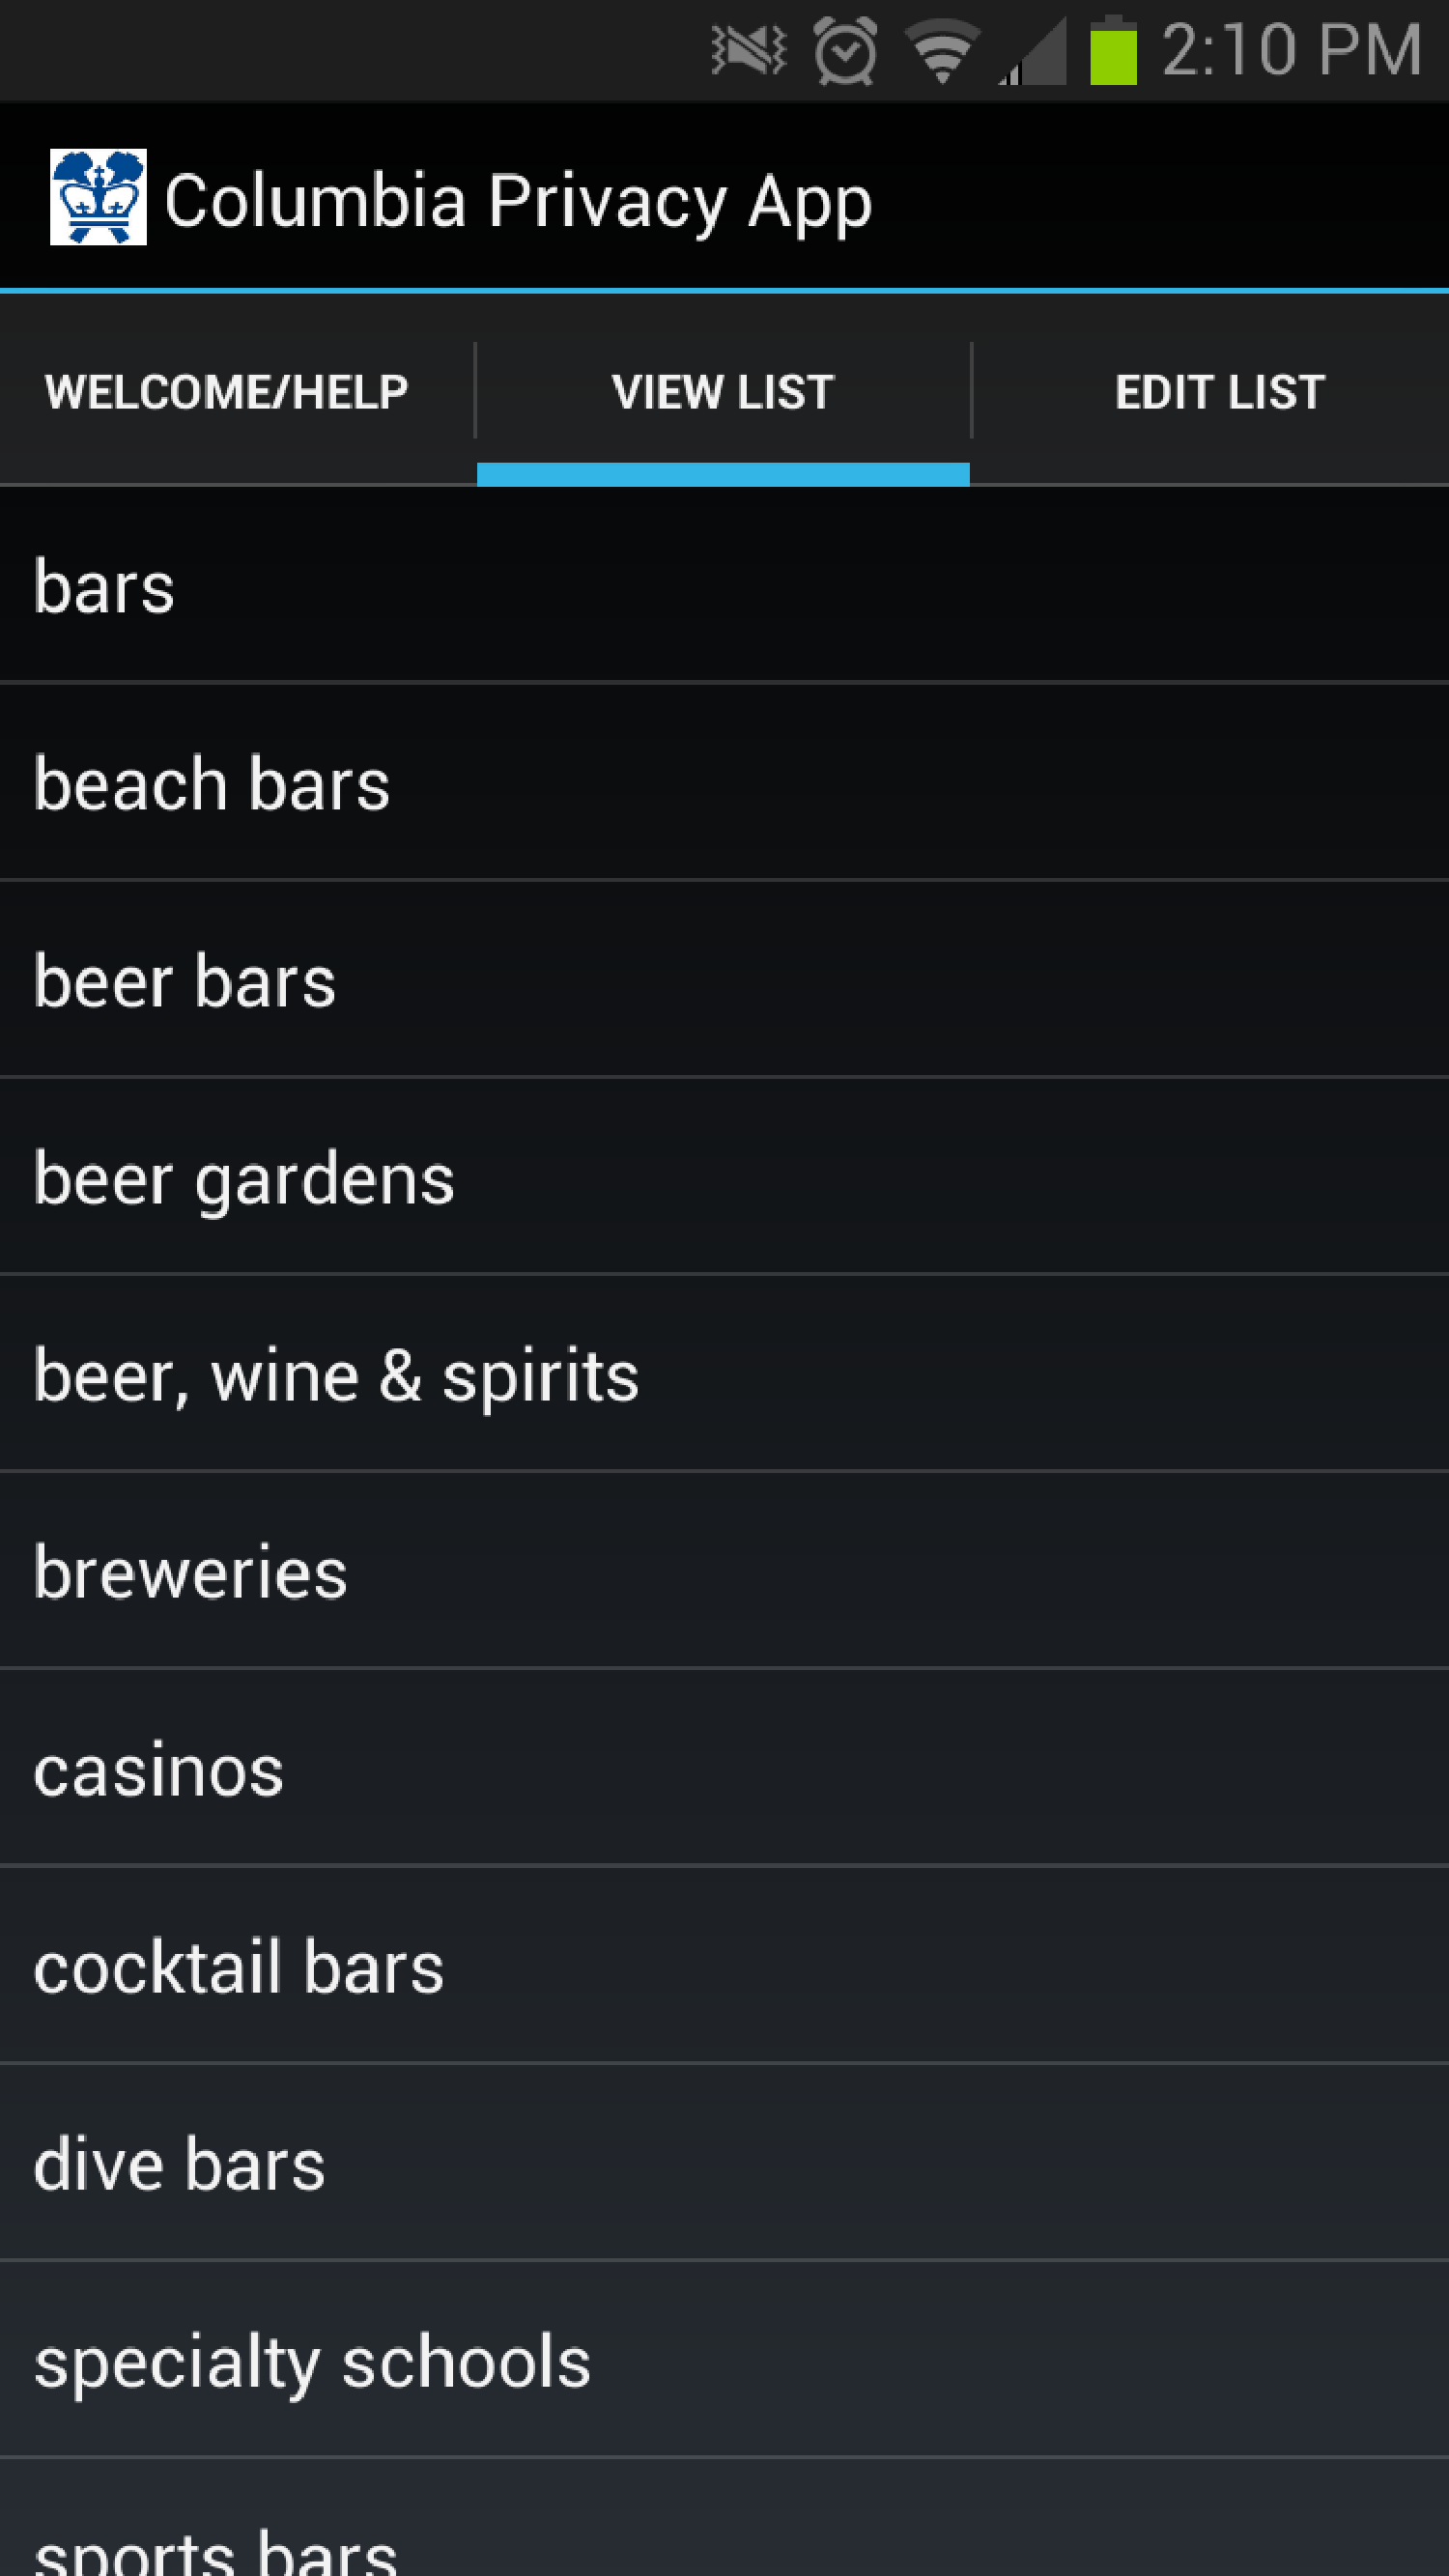
\includegraphics[width=0.75\linewidth]{./fig/screenshot_blacklist.pdf}
%   \caption{Blacklist}\label{fig:awesome_image1}
% \endminipage\hfill
\minipage{0.2\textwidth}
	\centering
  \includegraphics[width=0.75\linewidth]{fig/keyword/screenshot_addlist.pdf}
%  \caption{Adding screen}\label{fig:awesome_image2}
\endminipage\hfill
\minipage{0.2\textwidth}
	\centering
  \includegraphics[width=0.75\linewidth]{fig/keyword/screenshot_map.pdf}
%  \caption{Map}\label{fig:awesome_image3}
\endminipage
\caption{User Interface: (left) managing keywords black list, (right) visualizing locations released.}
\end{figure}
% \end{figure*}

% \begin{figure}[tbp]
% \centering
% \begin{tabular}[1]{cc}
% \hspace{-0.35cm}\includegraphics[width=0.75\linewidth]{./fig/screenshot_addlist.pdf}
% &
% \hspace{-0.35cm}\includegraphics[width=0.75\linewidth]{./fig/screenshot_map.pdf}
% \\
% (a) & (b) \\
% \end{tabular}
% \caption{(a) Blacklist addition screen (b) Map screenshot}
% \label{fig:awesome_image1}
% \end{figure}



% Server-- keywords and storage
% ISSUES: WHAT IF YELP DOESN'T HAVE A BUSINESS? what would a real impkementaiton look like?
% Our \textbf{webserver} had two main functions: reporting a location's keywords and storing a user's public location information.
% To map locations to keywords, we used the Yelp API. \texttt{Yelp.com} is an online ratings and review company.
% Yelp provides a hierarchical list of categories for all locations.~\footnote{Yelp categories: \url{http://bit.ly/12TyTER}}.
% Each time a device uploaded a lat-long to the server, we queried Yelp to find the categories of each location within 50 meters.
% This is a possible area for improvement; in future work, the radius of a query could change depending on an estimate of the device's current accuracy or a user's privacy preferences.
% The categories were then sent to the device.
% In a full implementation, this server should additionally be able to communicate with ad exchanges.

% For the purposes of our small scale user study, we did not create a \textbf{blocking module}. 
% In a full implementation, it would be necessary to block any third-party advertisers who did not participate in the system.
% The connections to ad-networks and aggregators (AdMob, Flurry Analytics etc.) can be blocked by a proxy in the middle and by spoofing the MAC address. 
% All necessary proxies already exist: Privoxy comes with advanced filtering capabilities and handles rewrites of the HTTP headers like the `referrer' header to prevent leakages of any form, and mitmproxy can handle SSL\footnote{\url{www.privoxy.org}, \url{www.mitmproxy.org}}. 
% In addition, as the system works with opt-in users, we can have the users upload their SSH certificates to enable the module in the middle to masquerade as the user. 
% From an application's perspective, no logic is broken. 
% Even for location based services like Foursquare or maps, an unintentional checkin or a search at a private location can be prevented by checking against the blacklist -- an added benefit.  

% Web interface
% The web interface, viewable at \url{keyword.cs.columbia.edu}, displayed all whitelisted locations, both on a map and listed with location keywords and times. In order to protect users' safety, users could contact us at any point if they were concerned about an unintentional location release. Additionally, any time a data point was recorded, we delayed making it public by 24 hours. Users could see their data points in real-time via a password-secured link.

% \begin{figure}[t]
% 	\begin{center}
% 		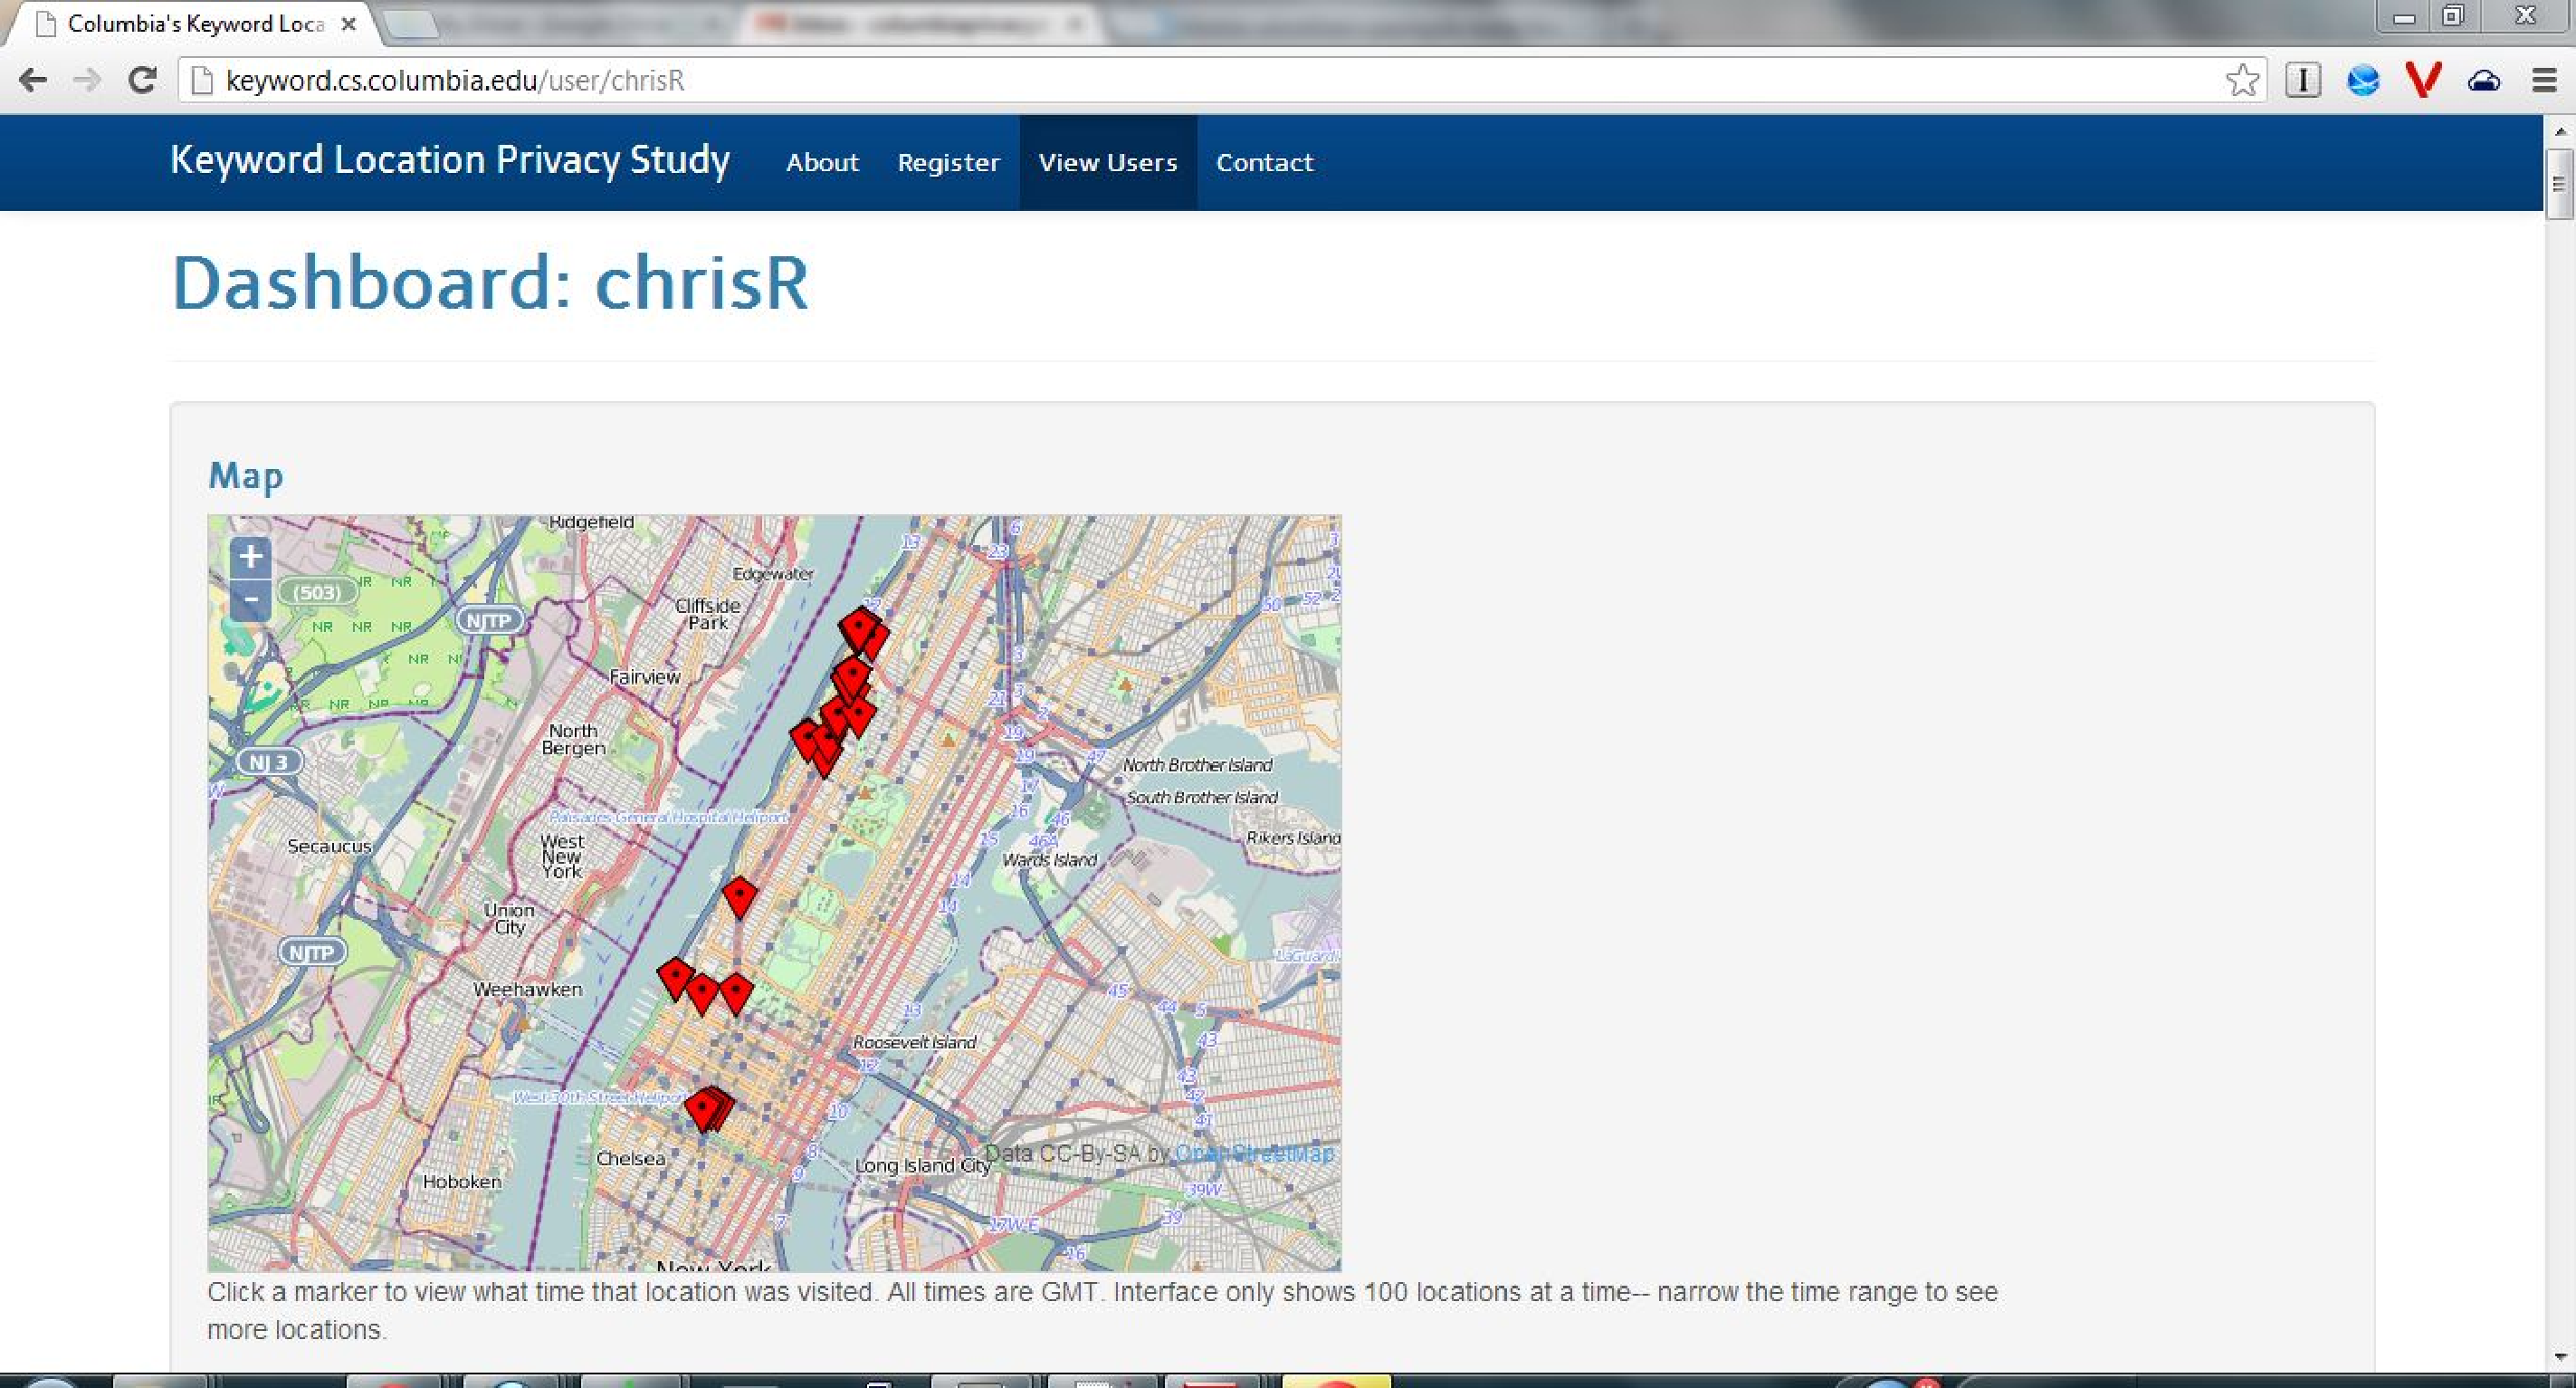
\includegraphics[width=0.9\linewidth]{./fig/web_map.pdf}
% 		% \subfigure[Map view]{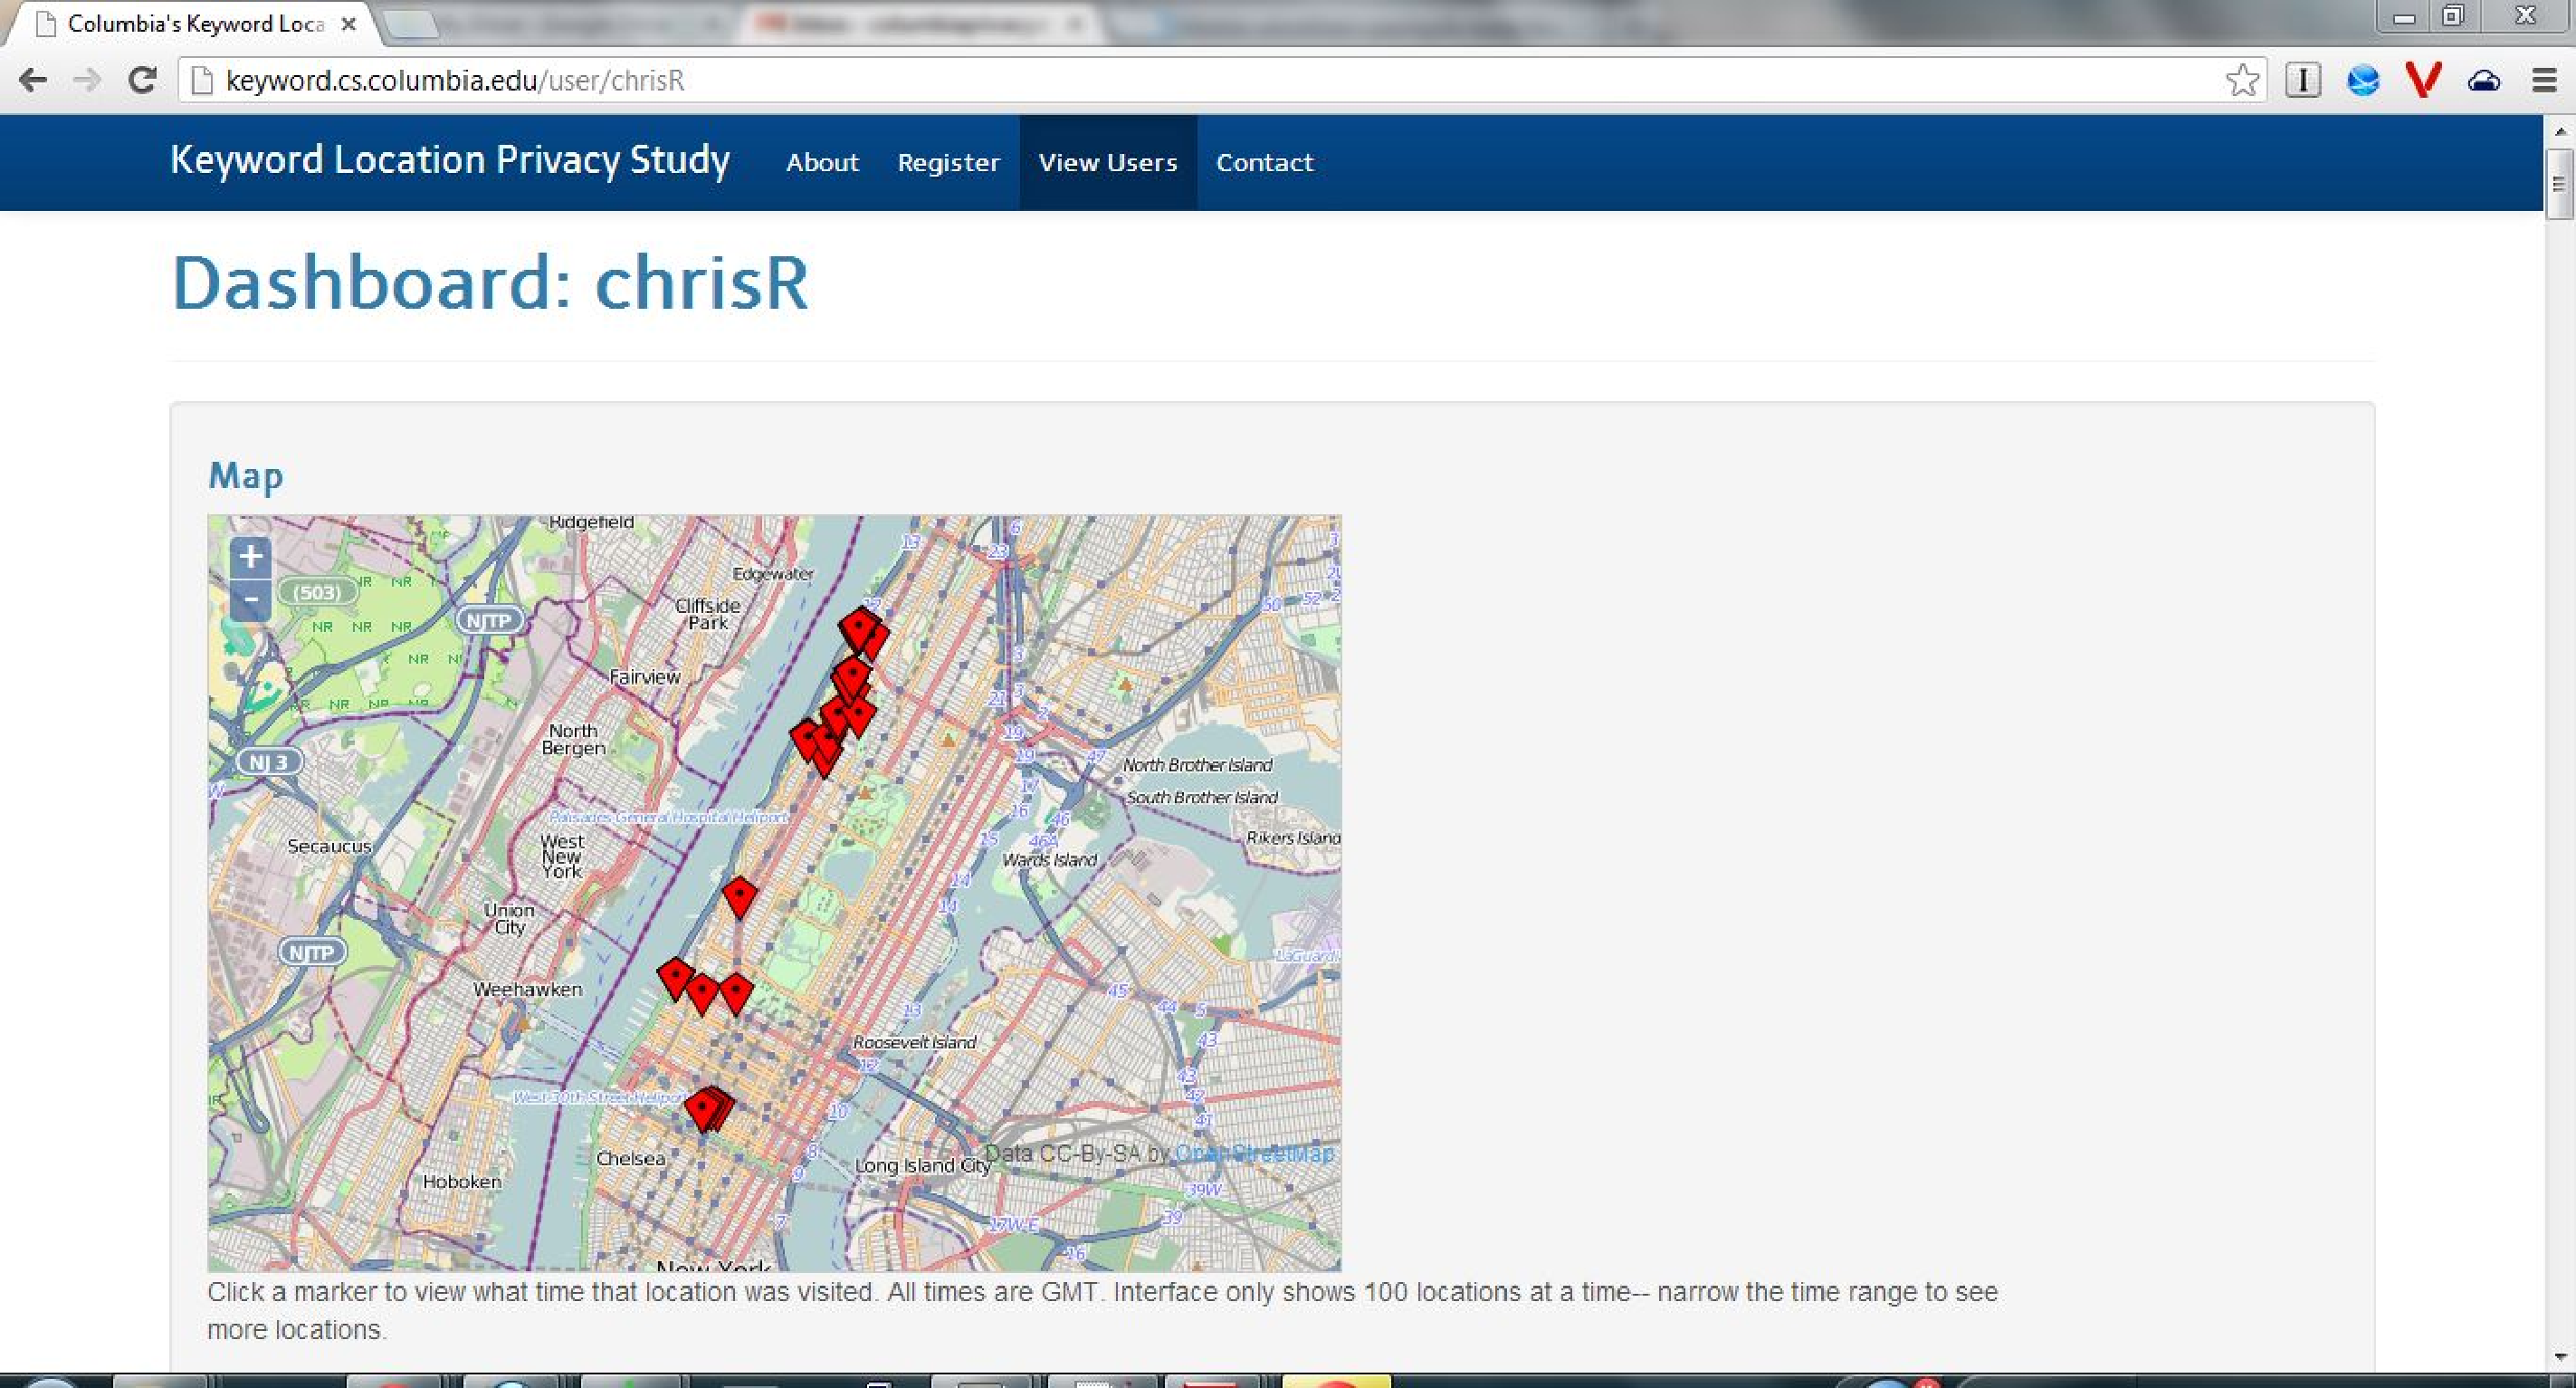
\includegraphics[width=0.9\linewidth]{./fig/web_map.pdf}}
% 		% \subfigure[List view]{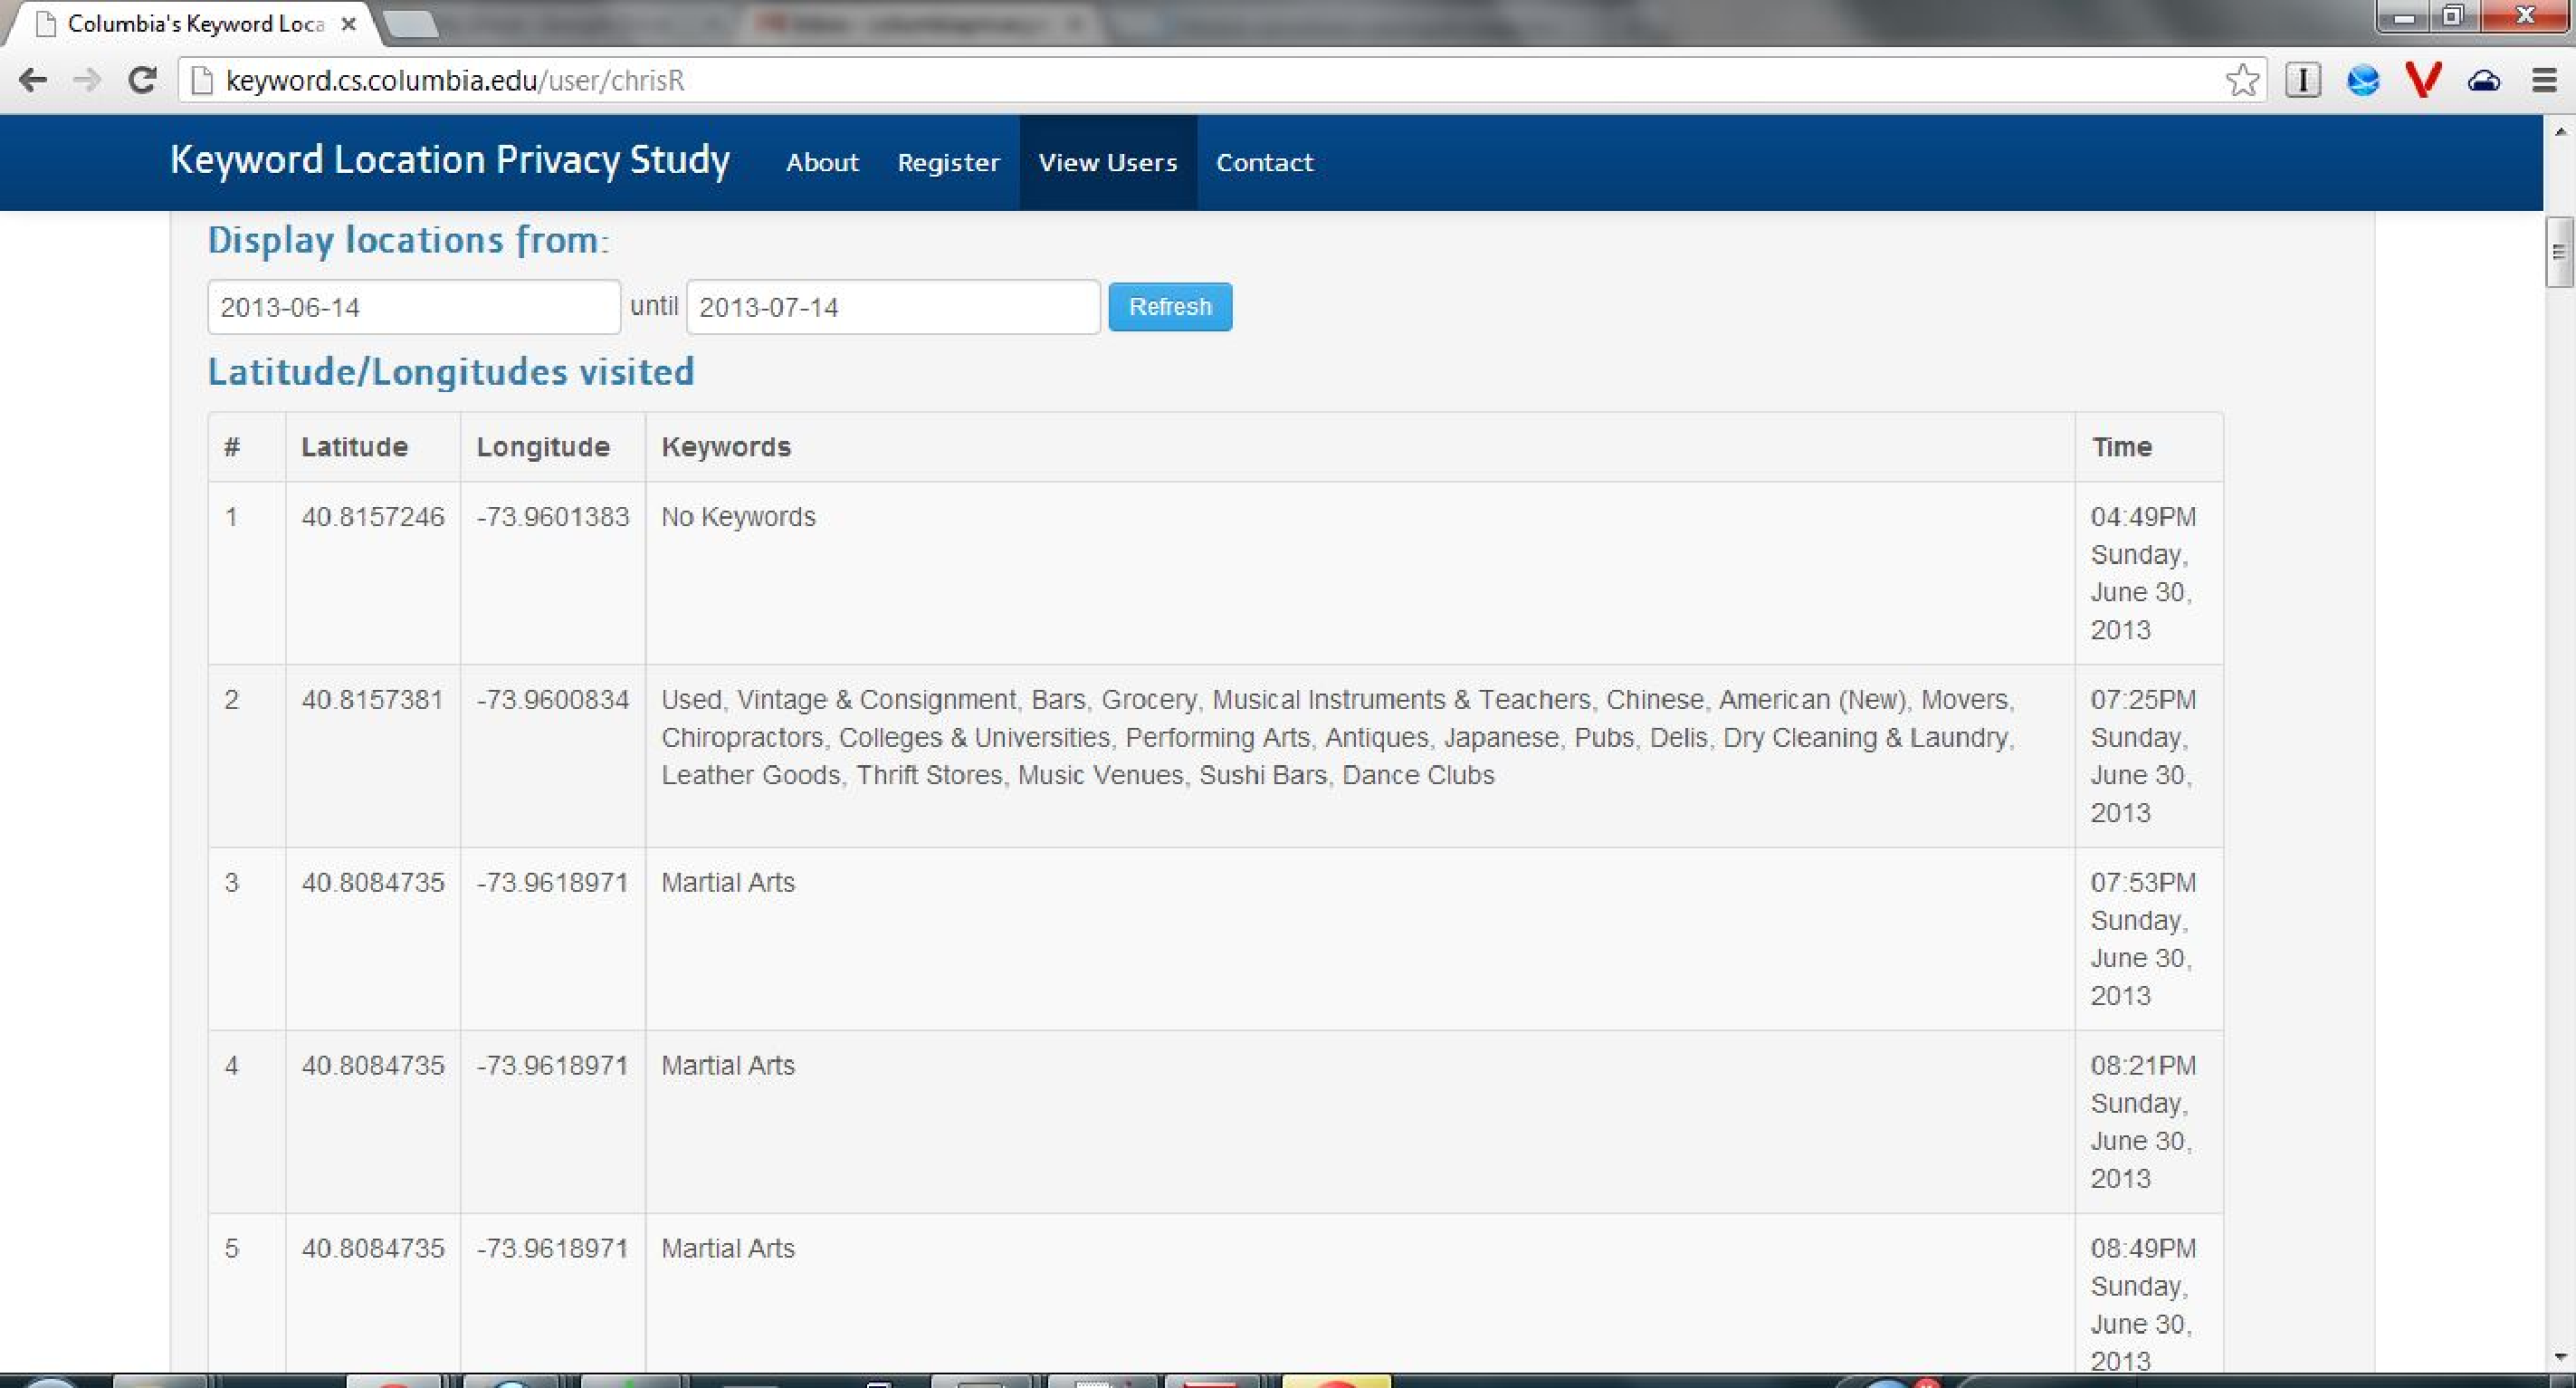
\includegraphics[width=0.9\linewidth]{./fig/web_list.pdf}}
% 	\end{center}
% 	\caption{Screenshot of our web interface (the data shown belong to an author, not a participant).}
% 	% \caption{Screenshot of web interface with one of the author's data. Top: map view. Bottom: list view.}
% 	\label{fig:webInterface}
% \end{figure}

% \subsection{Deployment}

% In a full implementation of our design, advertisers would pay a user whenever they showed an ad to her. 
% As this deployment was meant for exploratory purposes, we did not connect the system to any ad exchanges.
% We instead we simulated the incentives and costs a user might experience while using our system. 
% All participants received a small monetary sum for participating and were entered into a lottery.
% Each user was instructed that releasing more `valuable' information would give them a higher chance of the lottery.
% We did not disclose the exact method of valuing information, mimicking the opaque way in which information would be priced in a real implementation of the system. The intention was that this would incentivize users to release more information.
% % The incentive for a user to release information in our system is money. All participants received \$10 for participating. Additionally, we held a lottery among our users in which the winner would receive \$100. We instructed users that those whose information was more `valuable' would receive more `tickets' in the lottery, and would thus have a better chance of winning. We did not disclose the exact method of valuing information, mimicing the opaque way in which information would be priced in a real implemetation of the system. The intention was that this would incentivize users to release more information.
% To simulate the costs of disclosing information, we publicly displayed a user's non-blacklisted locations on a web interface.
% In a real system, a user would risk that her information is used improperly or released to those who might use it in a damaging way.
% We believed that publicly displaying a user's information accurately simulated this risk. 
% To increase the publicity of their information, we instructed users to post the link on a social media site, such as Facebook or Twitter, and email us a screenshot.

% We deployed our implementation with six users for two weeks. 
% Users were geographically diverse, located in multiple cities throughout the United States.
% % The users were geographically diverse within the USA, including cities on both coasts and the Midwest. 
% % The users were geographically diverse within the USA, including cities on both coasts and the Midwest. 
% Study participants were recruited through advertising on social networks and were primarily adults in their mid-twenties.

% instructions
\subsection{Deployment and Observations}
We deployed our implementation with six users for two weeks. 
Users were geographically diverse, located in multiple cities throughout the United States.
Study participants were recruited through advertising on social networks and were primarily adults in their mid-twenties.

After the study, we asked users to complete a survey. Our study was too small to make general conclusions, 
but we present results here to inform future work. 
% Users easily understood the keyword system and found the interface easy to use. 
Users easily understood both the keyword system and the interface. 
Users were divided on how well they felt the system secured their privacy, with some 
users concerned that our mapping of keywords to locations was not precise enough. Our users expressed a range of 
privacy sensitivities. Some did not use the blacklist and others used the blacklist to hide sites they associated with social stigma or that they thought would send negative signals to employers, insurers or the police.

% We next examined the (non-private) data of our users.
% There was a wide range in the number of locations released by each participant, easily explained by some using the blacklist more than others.
% After running the data through our valuation models, we also saw a wide range in the value across each user's data. 
% As in~\ref{subsec:eval}, we again analyzed the effect of blacklisting on ad revenue by valuing each user's data after removing potentially sensitive information.
% Note that in this case, the user may have already removed some sensitive locations.
% We found that the revenue loss was heterogenous across users: the categories with the largest losses, and the magnitudes of those losses, differed by user.
% When summed, the losses by category appeared to become smoother. This could suggest that a geographically diverse set of individuals will still maintain a good ad revenue despite privacy sensitivities. However, our sample size is to small to make such claims and we leave this question for future work.
